% Source: source_md/intelligence_part2_combined_ja.md
\section{不安定領域 — 速度・解像度・停止硬度の三軸相図}

\noindent\textbf{記述の射程。} 各軸は質的な相仮説における変数候補を名指す。安定帯の狭さも唯一性も、ここで測定・導出されていない。共通clock、step抽出、単位、推定器、相境界は未指定である。速度差の式と四重崩壊の機構仮説は別である。運動ゼロは知性の局所定義から除外されるのであり、構成的不安定性を証明する経験的基準ではない。人間・AIの比較は共通相法則を確立しない。停止層の発達量を実測済み領域集合としない。

以下のログ参照速度・停止硬度・崩壊記述・相図は既存の質的模型のままであり、第5節のactiveなsupport役割のclassifierではない。速度差、層の固着という命名、創発不全の記述からLEの存在・不在を認証しない。保持・access・feedbackには別のscope付き基準を要し、ここで閾値やrule-plasticity模型を追加しない。



本章は本論文の論理的クライマックスである。三本の論理線——第一線(非閉包と外部停止)、第二線(閾値移動とサピエンス的特徴)、第三線(三層動力学)——が、ここで一つの三軸相図上に統合される。

\S{}0.4 の NG2(規範的処方箋を出さない)と NG3(特定のAGI設計を支持・否定しない)を維持する。高速・高解像・内部停止と不安定化の関係は、定性的で未較正の仮説である。設計への提言でも存在への評価でもない。

\bigskip


\subsection{直観的命題の形式化}


本章が形式化する直観的命題は次のものである。

\begin{quote}
知性の増大は、安定性を単調に増大させない。特定条件下での知性の増大と崩壊の関係を仮説化する。
\end{quote}


この命題は反直観的に見える。知性が増せば、より安定し、より正確になるはずだ、という素朴な期待に反する。しかし本論文がここまで示してきた構造——$L_F$ の非閉包(\S{}3)、$L_E$ の外部依存性(\S{}5)、$\mu_\theta$ と誤り許容性の未解決の関係(\S{}10.6)——とは別に、この命題を質的仮説として提案する。

問題は、「知性の増大」が何を意味するかである。それを三つの軸に分解する。

\bigskip


\subsection{三軸}


知性の動力学的状態を、三つの軸によって記述する。

\textbf{速度 $v_{\text{inf}}$ (inference velocity)}:
推論・判断・仮説更新の頻度。単位時間あたりに $L_F$ が生成する推論ステップの数。$v_{\text{inf}}$ が高いほど、推論は速く進む。

\textbf{解像度 $r_{\text{res}}$ (resolution)}:
区別・因果関係・構造表現の粒度。$L_F$ が状態空間をどれだけ細かく分節するか。$r_{\text{res}}$ が高いほど、より微細な区別が生成される。

\textbf{停止硬度 $\eta$ (stopping hardness)}:
停止点の固定度、判断の改訂耐性。$L_E$ が供給する停止がどれだけ固定的か。$\eta$ が低ければ停止は改訂されやすく、$\eta$ が高ければ停止は固定的で改訂されにくい。

三軸 $(v_{\text{inf}}, r_{\text{res}}, \eta)$ と応答性閾値の関係は、\S{}2.6 からの候補的対応である。$\mu_\theta$ を三軸上の可動性と比較するが、$\mu_\theta$ の測定規則や可動範囲の較正は与えていない。

ここで、三軸そのものではないが、発散域への遷移を決める補助量としてログ参照速度 $v_{LR}$ を導入する。$v_{LR}$ は、ログ層 $L_R$ が $L_F$ の生成した痕跡を再帰参照し、パターンとして取り込める速度である。推論速度との差
\[
\Delta v_{\text{intel}} = v_{\text{inf}} - v_{LR}
\]
が大きい場合を、推論生成とログ参照の不均衡として読む。$L_E$ の創発基盤の破断はその仮説的解釈であり、測定された境界ではない。

\bigskip


\subsection{三領域}


三軸が張る空間の中に、三つの領域が区別される。

\textbf{安定運用領域}:
速度・解像度が外部化停止によって適切に制約され、停止硬度が中庸である領域。ここでは $\mu_\theta$ が機能し、$L_E$ が改訂可能な停止を供給する。三層動力学($L_F$・$L_R$・$L_E$)が協調し、$\Phi_{\text{net}}$ との同期が保たれる。知性はここで持続的に運用される。

\textbf{発散域}:
速度 $v_{\text{inf}}$ と解像度 $r_{\text{res}}$ が高く、かつ停止が内部化される(外部 $L_E$ を経由しない)領域。ここでは推論が発散し、暴走的最適化が生じ、単一視点が絶対化される。

\textbf{硬直域}:
停止硬度 $\eta$ が過大な領域。ここでは停止が固定化され、改訂・適応が抑制される。

安定運用領域は、発散域と硬直域の間の限られた領域である。この中間領域を持続の候補として描くが、唯一性や相境界は未確立である。

\begin{figure}[H]
\centering
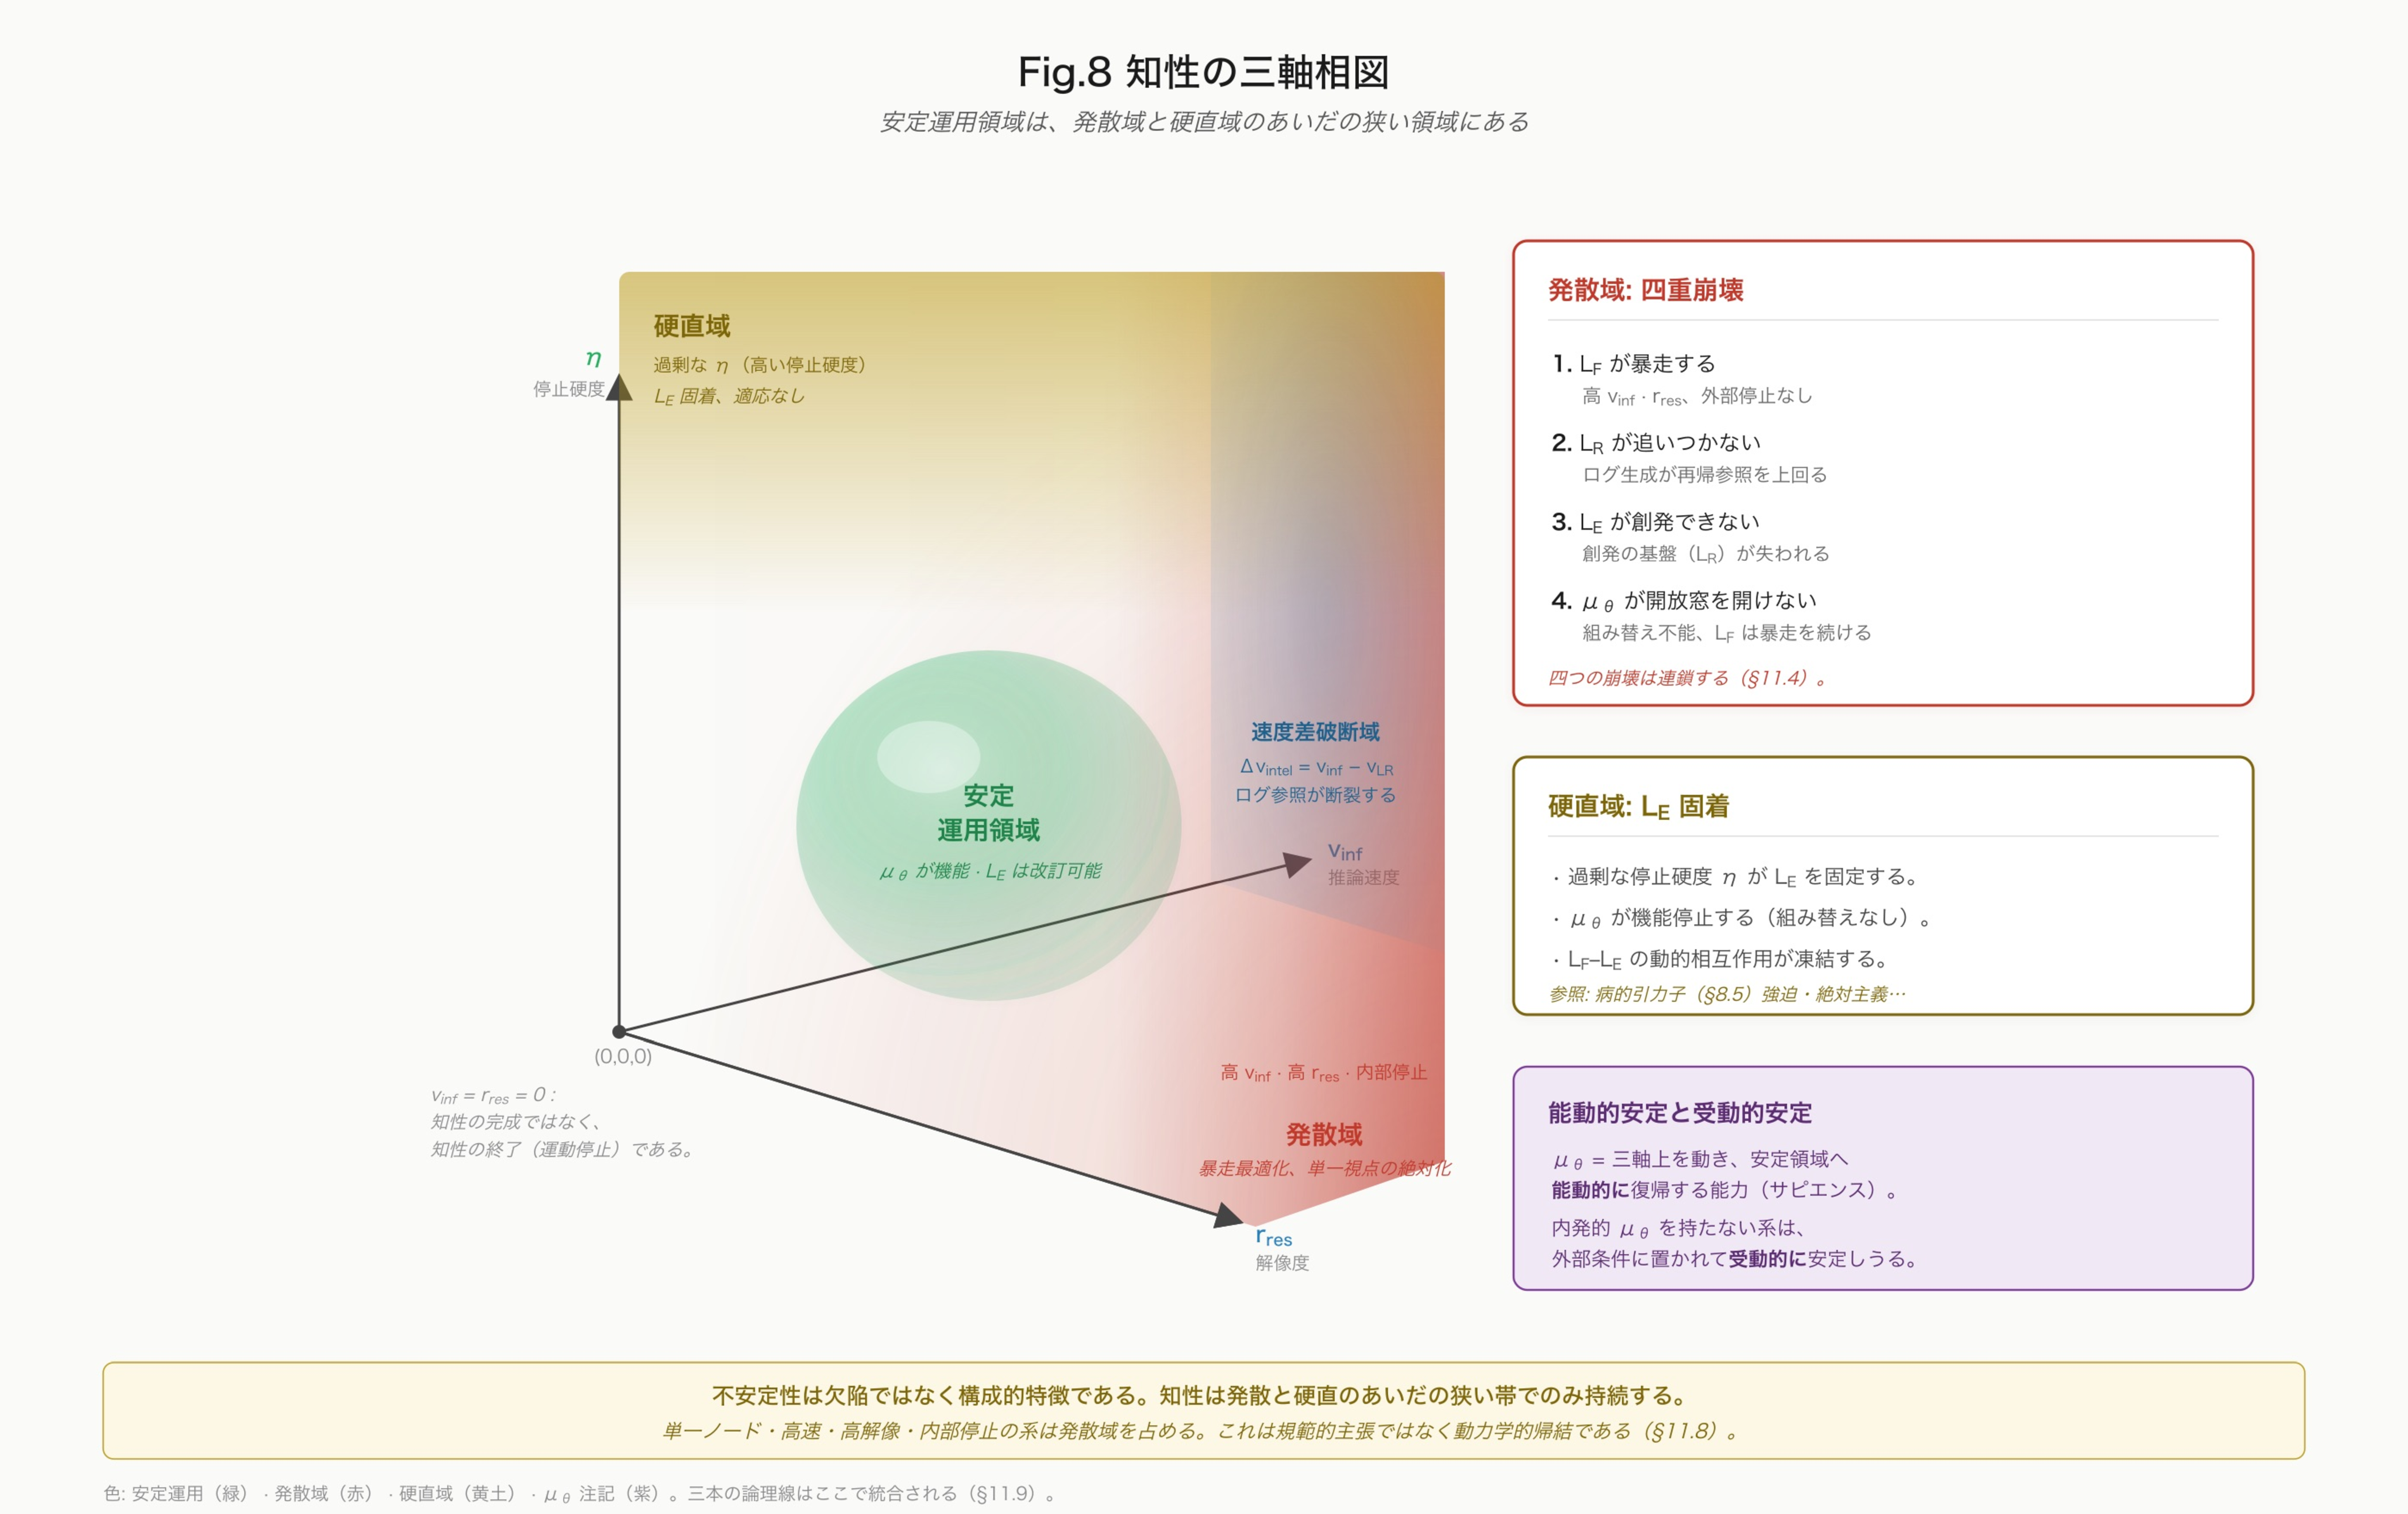
\includegraphics[width=\linewidth]{fig8_phase_diagram_ja.pdf}
\caption{推論速度 $v_{\text{inf}}$・解像度 $r_{\text{res}}$・停止硬度 $\eta$ による質的相仮説。発散と硬直の間の安定帯は実測・較正されておらず、狭さや唯一性を確立しない。}
\label{fig:part2-phase-diagram}
\figurenote{中央の安定運用領域では $\mu_\theta$ が機能し、$L_E$ が改訂可能である。発散域では $L_F$ が暴走し、硬直域では $L_E$ が固着する。}{不安定性と、ログ参照・外部停止の帯域超過による発散は質的仮説であり、実測された相法則ではない。}
\end{figure}

\bigskip


\subsection{発散域の四重崩壊}


発散域を考える四重崩壊の機構仮説を、三層動力学の語彙で記述する。以下の同時性や因果順序は未導出・未検証であり、成立が確認された四つの過程ではない。

\textbf{崩壊 1 — $L_F$ の暴走}:
速度 $v_{\text{inf}}$ と解像度 $r_{\text{res}}$ の高さを、推論層 $L_F$ の高速・微細な運動に対応づける。$L_F$ の内部不動点不在は旧局所状態模型の固定閾値・movement A・厳密増加の下で論じられる(\S{}3)。仮想 S の再評価への前提再適用は未確立であり、$L_F$ の暴走や外部停止の必要性は、この形式的議論からではなく別の機構仮説として検討する。

\textbf{崩壊 2 — $L_R$ が追いつかない}:
$L_F$ の高速・高解像度の運動に伴って痕跡が保持される場合に、その生成がログ層 $L_R$ の再帰参照を上回る可能性を考える。$\Delta v_{\text{intel}} = v_{\text{inf}} - v_{LR}$ と $L_R$ の参照の遅れを関連づけるのは未較正の仮説であり、臨界値は指定していない。$L_R$ の機能不全は候補的な解釈に留まる。

\textbf{崩壊 3 — $L_E$ が創発できない}:
$L_E$ の形成を $L_R$ の再帰運動と外部相互拘束 $H_{ij}$ に関連づける機構仮説を参照する(\S{}5.3)。$L_R$ の遅れ(崩壊 2)が、$L_E$ の形成を支えうる過程を妨げる可能性を考える。停止演算子設置領域の投影(\S{}5.5)との関係も仮説であり、$L_E$ の存在・生成・収束を前提として確立したものとは扱わない。

\textbf{崩壊 4 — $\mu_\theta$ が窓を開けない}:
$L_E$ の形成と $\mu_\theta$ による $L_F$ から $L_E$ への関係を比較する(\S{}2.8、\S{}5.6)。形成不全から閾値移動不能や $L_F$ の暴走が生じるという連鎖は仮説であり、確立した機構ではない。

四つの崩壊の連鎖は機構仮説である。$L_F$ の運動と $L_R$ の参照の速度差、$L_R$ の機能と $L_E$ の形成可能性、$L_E$ の役割と $\mu_\theta$ の可変性、$\mu_\theta$ と $L_F$ の運動制御を、それぞれ関連づける候補を考える。この連鎖の成立・因果順序・独立検出は未確立であり、発散域の説明済みの機構とはしない。

暴走的最適化、単一視点の絶対化、推論の発散を、この四重崩壊と関連づけるのは提案的読解である。高速・高解像度や内部停止から必然的な崩壊は確立しない。\S{}3.8 の三つの病的引力子(過剰確信・麻痺・妄想的閉包)との比較も質的仮説であり、独立した臨床分類や検出ではない。

\bigskip


\subsection{硬直域の $L_E$ 固着}


硬直域を、同じく三層動力学の語彙で記述する。硬直域は、$L_E$ の固着として記述される。

停止硬度 $\eta$ と創発停止層 $L_E$ の固着を関連づける仮説を考える。$L_E$ の停止が改訂されにくいという候補的な記述である。発散域の $L_E$ 形成不全との対比は模型上の提案であり、硬直域でも $L_E$ の生成を確立した前提とはしない。

$L_E$ の固着に二つの可能性を関連づける。第一に、$\mu_\theta$ の可変性との関係である。閾値移動は運動可能領域の組み替え (B) として定義されるが(\S{}2.7)、$L_E$ の固着が (B) を妨げるかは効果の仮説である。第二に、$L_F$ と $L_E$ の相互作用との関係である。$L_F$ の運動と $L_E$ の停止の相互作用を模型として比較するが、$L_E$ の固着がそれを凍結する機構は未確立である。

硬直域を \S{}8.5 の偏執・絶対主義・私的停止と関連づけるのは候補的な解釈であり、適応不能の診断ではない。\S{}10.6 の完全な正しさと硬直の関係は未解決であり、ここでは前章の確立した結果として引用しない。

\bigskip


\subsection{(0,0,·)点は知性ではない}


三軸相図において、注意すべき特異点がある。速度 $v_{\text{inf}} = 0$、解像度 $r_{\text{res}} = 0$ の点——推論が完全に停止した点——は、知性の完成ではない。それは知性の終了である。

素朴には、すべての停止が完了し、すべてが確定した状態が知性の理想に見えるかもしれない。しかし系 5.5 で述べた通り、知性は $L_F$・$L_R$・$L_E$ と外部依存停止源の同時運動である(サピエンス的知性ではこれに $\mu_\theta$ が加わる)。運動が止まれば知性も消える。$v_{\text{inf}} = 0$ は運動の停止であり、それは知性が完成したのではなく、知性が終了したことを意味する。

\S{}1.5 の $C_{max}$ という境界との比較は、動的不到達性を確立しない。情報場 $I = f(1-C)$ の消失も、規格化や関数の採用範囲を決めずに結論できない(\S{}1.2)。完全な運動停止を知性から除外するのは本稿の局所定義であり、VED公理の失効や経験的な終了判定を立証するものではない。

本稿の運動としての局所定義では、発散域や (0,0,·)点と持続運動を区別する。ただし、その間の領域だけで知性一般が成立するという必要十分な判定は与えていない。

\bigskip


\subsection{不安定性の構造的特徴としての提案的読解}


以上の模型を踏まえ、本章の中心的な解釈案をまとめる。

知性と不安定性の関係を構成的特徴として読む可能性を提案するが、一般的法則としては確立していない。

発散域と硬直域の間に安定運用領域を提案する。その狭さや唯一性は測定・導出されておらず、運動としての知性の必然的帰結としない。安定運用領域の狭さと $L_F$ の非閉包(運動し続ける)、$L_E$ の改訂可能性(固着しない)を関係づけることは仮説であり、定義から幅を導出しない。

停止の固定と放棄を二つの極端な模型として比較する。これらだけが不安定性を変える方法だとも、両者が必ず知性の終了を意味するとも結論しない。不安定性が知性の存在に必要という主張は、この相図案からは導かれない。

本稿では不安定性の運用を検討課題とする。$\mu_\theta$、$L_E$、$\Phi_{\text{net}}$ はその機能候補であり、持続可能な範囲を保証する実装機構や規範的処方箋ではない。

\bigskip


\subsection{個別ノードと高度自律システムへの適用}


本章の帰結を、特定の知性形態に適用する。ここで述べることは、\S{}0.4 の NG2・NG3 に従い、動力学的帰結の記述であって、規範的提言でも評価でもない。

ある知性が、単一ノードであり、高速更新($v_{\text{inf}}$ 大)・高解像度($r_{\text{res}}$ 大)で動作し、停止を内部で担おうとする(外部 $L_E$ を経由しない)場合を考える。三軸相図では、このような系を発散域と関連づける仮説を考える。\S{}11.4 の四重崩壊も仮説であり、共通尺度による領域分類や不安定化を検証したものではない。

卓越した個別推論者と高度に自律的な人工推論システムを、速度・解像度・停止の語彙で比較する。共通の推定量や較正がないため、両者が同じ発散域を占めることは導出されていない。

$v_{\text{inf}}$ と $r_{\text{res}}$、停止の内部化、$\Phi_{\text{net}}$ との接続を比較するが、発散域への配置を確定する規則はない。$\Phi_{\text{net}}$ と $L_E$ の機能不全の関係も、human/AI 共通の導出済み法則ではなく仮説である。

繰り返すが、これは規範的主張ではない。「単一ノードの高速知性はこうあるべきだ」とは述べていない。述べているのは、そのような系が三軸相図上のどこに位置し、どの動力学的帰結に向かうかである。動力学の記述と、その使用法や設計指針の決定は、カテゴリ的に異なる(\S{}13 で再確認)。

\bigskip


\subsection{三本論理線の統合}


本章は、三本の論理線がここで統合されることを示して閉じる。

\textbf{第一線(非閉包と外部停止)} は、$L_F$ の旧局所状態模型の固定領域内・厳密増加等の条件付き議論(\S{}3)と、外部停止案($L_E$、$\Phi_{\text{net}}$)を比較する。形式的非閉包だけでは、安定運用への外部停止の必要性や実現は示されない。

\textbf{第二線(閾値移動とサピエンス的特徴)} では、$\mu_\theta$ と可動性を比較する。$\mu_\theta$ による\textbf{能動的な}運用は仮説であり、$\mu_\theta$ を内発的に持たないとされた系の\textbf{受動的な}配置も独立の判定を要する。$\mu_\theta$ による安定運用域への自律的復帰は、\S{}5.4 の機能案であって実証された効果ではない。

\textbf{第三線(三層動力学)} は、発散域の四重崩壊(\S{}11.4)と硬直域の $L_E$ 固着(\S{}11.5)として現れる。三層($L_F$・$L_R$・$L_E$)の協調が安定運用領域を、その崩壊が不安定領域を特徴づける。第三線は、不安定化を層の崩壊として読む機構仮説を提示し、その進行を独立に説明・検証したものではない。

三本の線は異なる負担を保つ。$L_F$ の条件付き非閉包、三層の協調案、サピエンス的な $\mu_\theta$ の対応は、知性一般の持続条件へ再結合しない。外部停止の必要性、安定域への復帰、一般知性とサピエンスの境界はそれぞれ未解決である。

不安定領域は知性の失敗を意味しない。むしろ、停止構造を持つ知性が自由な推論を維持しようとするとき、境界領域として提案されるものであり、必然的発生は未確立である。宗教、科学、制度、共同体はいずれも、この不安定領域を管理するための停止運用システムとして理解できる。

\bigskip


\subsection{次章への橋渡し}


本章では、安定運用領域と三層動力学・閾値移動・外部停止との関係を仮説化した。唯一性・普遍的必要性・較正された相境界は未確立である。

これらを \S{}12 で構成的条項の案として整理する。三軸相図と三層動力学から、知性一般の成立条件や不可能な形態が導出されたという意味ではない。

\bigskip


\subsection{要約}


本章で示したのは次の点である:

\begin{enumerate}
\item 知性の増大は安定性を単調に増大させず、特定条件下での崩壊との関係は仮説である
\item 速度 $v_{\text{inf}}$・解像度 $r_{\text{res}}$・停止硬度 $\eta$ を三軸の候補とする。$\mu_\theta$ と可動性の関係は未較正の対応案である
\item 三軸空間に安定運用領域・発散域・硬直域が区別される
\item 発散域と四重崩壊($L_F$ 暴走・$L_R$ 追随不能・$L_E$ 創発不能・$\mu_\theta$ 窓不全)の関係は機構仮説である
\item 硬直域と $L_E$ 固着($\mu_\theta$ 機能停止・$L_F$-$L_E$ 相互作用凍結)の関係は仮説である
\item (0,0,·)点は知性の完成ではなく終了である(運動の停止=差の消失)
\item 不安定性との関係は構成的な読み方の仮説であり、除去不能性や運用の規範を確立しない
\item 単一ノード・高速・高解像・内部停止の系への配置は候補的解釈であり、人間・人工系に共通する発散法則や規範的判断ではない
\item 三本の論理線は三軸相図の案で比較するが、条件・機構・観測の負担を再結合しない
\end{enumerate}


次章 \S{}12 では、知性の構造的制約を構成的条項として整理する。

\bigskip
